\chapter{Resultados Experimentais} \label{cpt:result}
Neste capítulo, são apresentados os resultados obtidos pelo modelo de simulação em diferentes contextos. Serão comparados os resultados de três simulações em configurações de ambientes distintos, porém com o mesmo tempo total de simulação, i.e., o mesmo número de passos de simulação, totalizando 12 passos, configurados em um período de 3 dias, com duração de 4 horas cada. Por fim, é feita uma demonstração dos resultados do modelo de geração de textos médicos a partir da API da OpenAI.

\section{Simulação 1}\label{sec:simul1}
Para a primeira simulação, considerou-se uma configuração do ambiente com apenas um hospital e com uma chegada de pacientes moderada considerando a capacidade total dos leitos. Foi escolhido o hospital HEPA, localizado no bairro Teresópolis e com as seguintes configurações de leitos:

\begin{itemize}
    \item ``Psquiatria'' do tipo ``Outras Especialidades'' contendo um total de 264 leitos, sendo 159 leitos SUS;
    \item ``Saúde Mental'' do tipo ``Hospital Dia'' contendo um total de 15 leitos, sendo os 15 leitos SUS.
\end{itemize}

Para fins de teste do modelo de simulação, para a especialidade ``Psiquiatria'', foi considerado um total de 500 internações durante o período de simulação, das quais 300 das internações são alocadas em leitos do SUS. Também foi informado que cada paciente ocupará, em média, de 1 a 4 passos de simulação enquanto estiver no leito hospitalar. Na especialidade ``Saúde Mental'', considera-se a ocorrência de 50 internações, das quais todas as 50 são em leitos do SUS. Nessa especialidade, os pacientes também permanecerão internados por um intervalo de 1 a 4 passos de simulação. A Figura~\ref{fig:simul-config-1} apresenta um recorte da configuração do ambiente na interface gráfica.

\begin{figure}
    \centering
    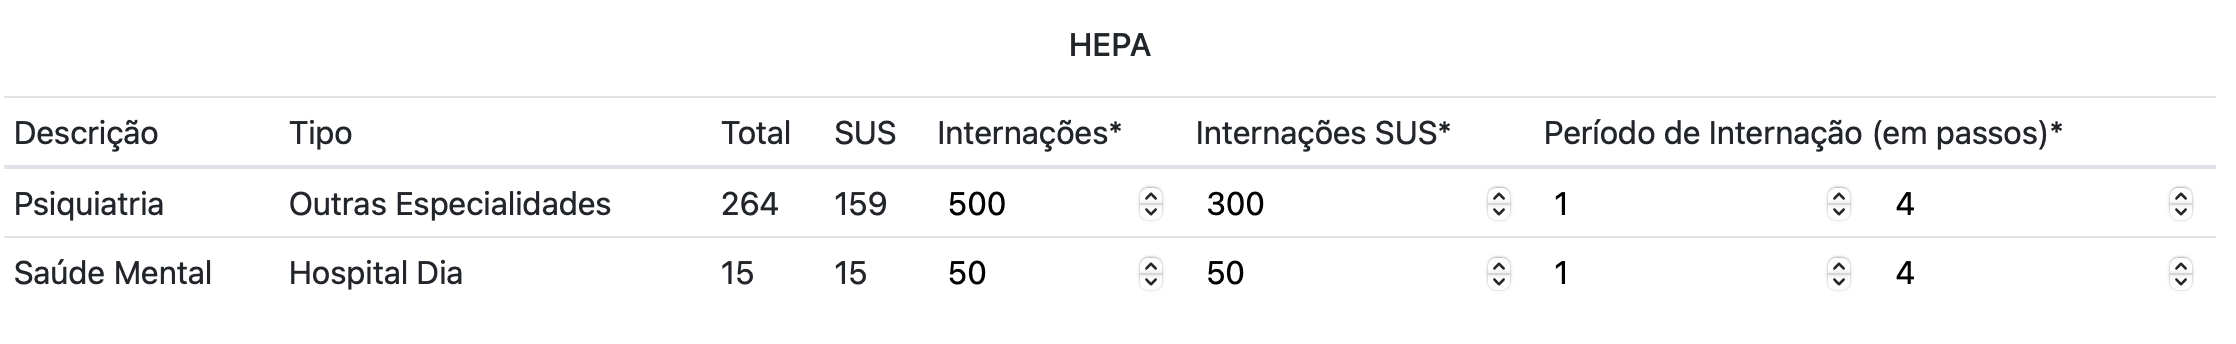
\includegraphics[width=\textwidth]{Capitulos/images/simul-config-1.png}
    \caption{Configuração dos leitos do hospital HEPA na simulação.}
    \label{fig:simul-config-1}
\end{figure}

Após a execução da simulação no contexto apresentado anteriormente, o resultado demonstrou que durante o período informado, e com os parâmetros selecionados, o leito da especialidade ``Psiquiatria'' não chegou a sua lotação máxima. No entanto, o leito da especialidade ``Saúde Mental'' passou da capacidade total de leitos no décimo primeiro passo de simulação, caracterizando uma superlotação no setor, isso se deu devido ao fluxo de entrada e saída dos pacientes nos leitos do hospital. As Figuras~\ref{fig:simulacao1-ocupacao1} e \ref{fig:simulacao1-ocupacao2} mostram o estado dos leitos em cada um dos passos de execução da simulação. As linhas em azuis nos gráficos representam a quantidade de leitos sendo utilizados no passo de simulação e as linhas em amarelo a capacidade de leitos daquela especialidade no hospital.

%GA: a tabela abaixo poderia ser um grafico de linhas, com uma linha para cada hospital (e pontilhada para SUS, por exemplo). (GV: corrigido)
%GA: também poderia ter o plot do limite de leitos como uma linha na horizontal (GV: corrigido)
%GA: acho que ficou melhor como grafico de linhas do que a tabela. Talvez não seja um problema os eixos Y n serem alinhados por não ser a mesma disponibilidade de leitos, mas é uma boa confirmar com a Soraia

\begin{figure}
\centering
\begin{subfigure}{0.49\textwidth}
    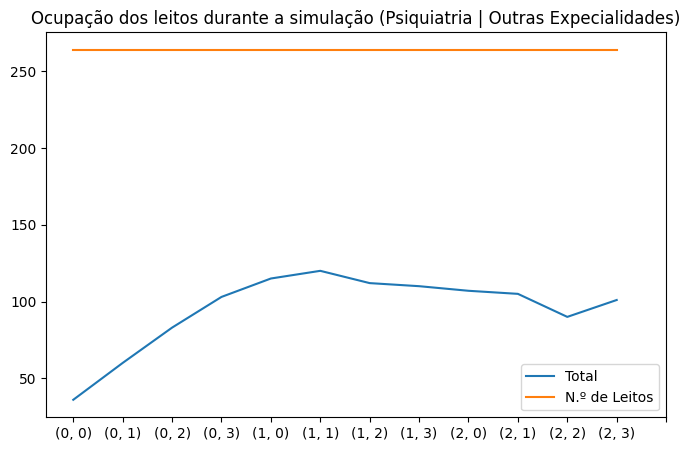
\includegraphics[width=\textwidth]{Capitulos/images/simul-psi-1.png}
    \caption{Ocupação dos leitos.}
\end{subfigure}
\hfill
\begin{subfigure}{0.5\textwidth}
    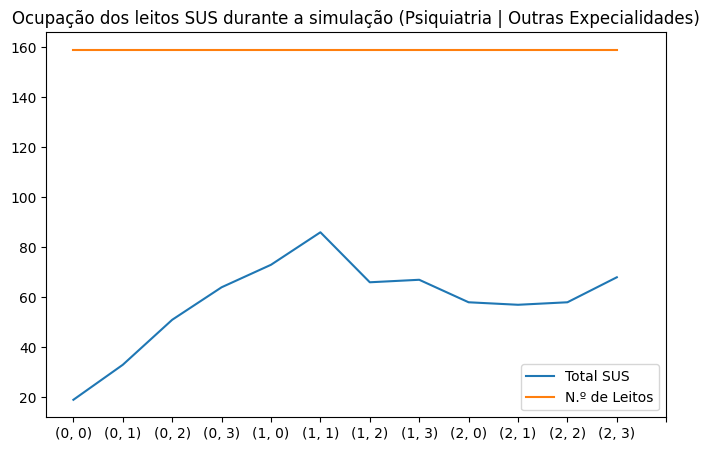
\includegraphics[width=\textwidth]{Capitulos/images/simul-psi-2.png}
    \caption{Ocupação dos leitos SUS.}
\end{subfigure}
        
\caption{Ocupação dos leitos durantes os passos de simulação para a especialidade ``Psquiatria'' do tipo ``Outras Especialidades'' do hospital HEPA.}
\label{fig:simulacao1-ocupacao1}
\end{figure}

\begin{figure}
    \centering
    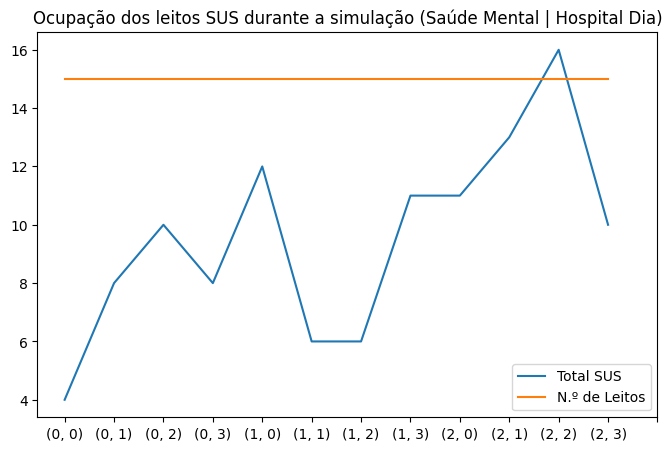
\includegraphics[width=0.5\textwidth]{Capitulos/images/simul-mental.png}
    \caption{Ocupação dos leitos SUS durantes os passos de simulação para a especialidade ``Saúde mental'' do tipo ``Hospital Dia'' do hospital HEPA.}
    \label{fig:simulacao1-ocupacao2}
\end{figure}

% \begin{table}[h!]
% \centering
% \begin{tabular}{ |l|l|l|l| } 
%  \hline
%  Passo & Leito & Total & Total SUS \\ 
%  \hline
%  1 & Psiquiatria - Outras Especialidades & 36 & 19\\  \hline
%  1 & Saúde Mental - Hospital Dia & 4 & 4\\  \hline
%  2 & Psiquiatria - Outras Especialidades & 60 & 33\\  \hline
%  2 & Saúde Mental - Hospital Dia & 8 & 8\\  \hline
%  3 & Psiquiatria - Outras Especialidades & 83 & 51\\  \hline
%  3 & Saúde Mental - Hospital Dia & 10 & 10\\  \hline
%  4 & Psiquiatria - Outras Especialidades & 103 & 64\\  \hline
%  4 & Saúde Mental - Hospital Dia & 8 & 8\\  \hline
%  5 & Psiquiatria - Outras Especialidades & 115 & 73\\  \hline
%  5 & Saúde Mental - Hospital Dia & 12 & 12\\  \hline
%  6 & Psiquiatria - Outras Especialidades & 120 & 86\\  \hline
%  6 & Saúde Mental - Hospital Dia & 6 & 6\\  \hline
%  7 & Psiquiatria - Outras Especialidades & 112 & 66\\  \hline
%  7 & Saúde Mental - Hospital Dia & 6 & 6\\  \hline
%  8 & Psiquiatria - Outras Especialidades & 110 & 67\\  \hline
%  8 & Saúde Mental - Hospital Dia & 11 & 11\\  \hline
%  9 & Psiquiatria - Outras Especialidades &107 & 58\\  \hline
%  9 & Saúde Mental - Hospital Dia & 11 & 11\\  \hline
%  10 & Psiquiatria - Outras Especialidades & 105 & 57\\  \hline
%  10 & Saúde Mental - Hospital Dia & 13 & 13\\  \hline
%  11 & Psiquiatria - Outras Especialidades & 90 & 58\\  \hline
%  11 & Saúde Mental - Hospital Dia & 16 & 16\\  \hline
%  12 & Psiquiatria - Outras Especialidades & 101 & 68\\  \hline
%  12 & Saúde Mental - Hospital Dia & 10 & 10\\  \hline
% \end{tabular}
% \caption{Estados dos leitos hospitalares para cada passo de simulação.}
% \label{table:result1}
% \end{table}

A Figura~\ref{fig:simul-result-1} ilustra alguns dos estados da ocupação dos leitos do hospital HEPA na interface gráfica. A Figura~\ref{fig:simul-result-1}(a) apresenta o estado do hospital após o final da execução do primeiro passo de simulação, com 14.34\% do total de leitos hospitalares ocupados, e a Figura~\ref{fig:simul-result-1}(b) demonstra esses dados após o final da execução do ultimo passo de simulação, com 39.78\% do total dos leitos hospitalares ocupados.

\begin{figure}
\centering
\begin{subfigure}{0.8\textwidth}
    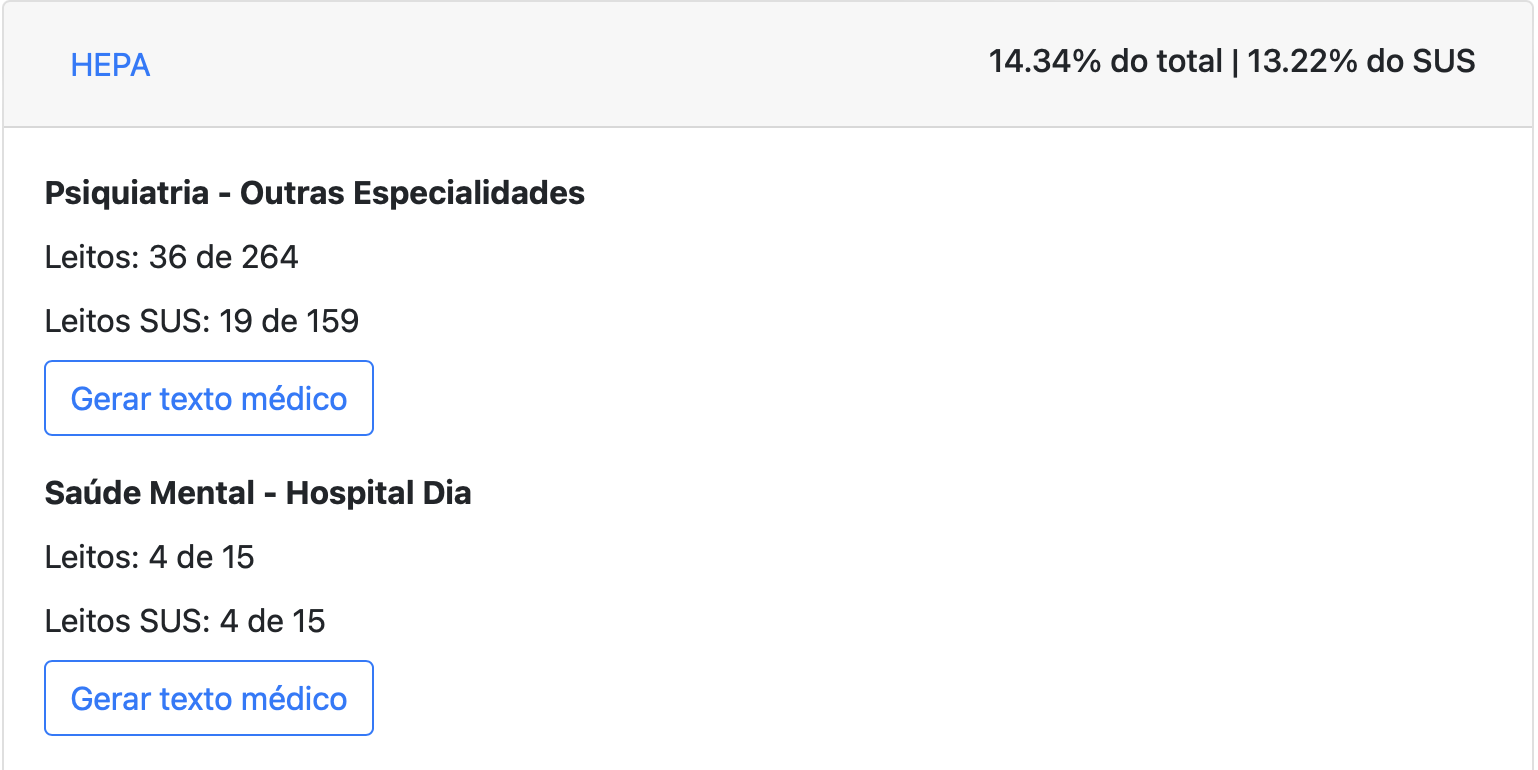
\includegraphics[width=\textwidth]{Capitulos/images/simul-result-1a.png}
    \caption{Estado dos leitos do hospital HEPA ao final do primeiro passo de simulação.}
    \label{fig:first}
\end{subfigure}
\hfill
\begin{subfigure}{0.8\textwidth}
    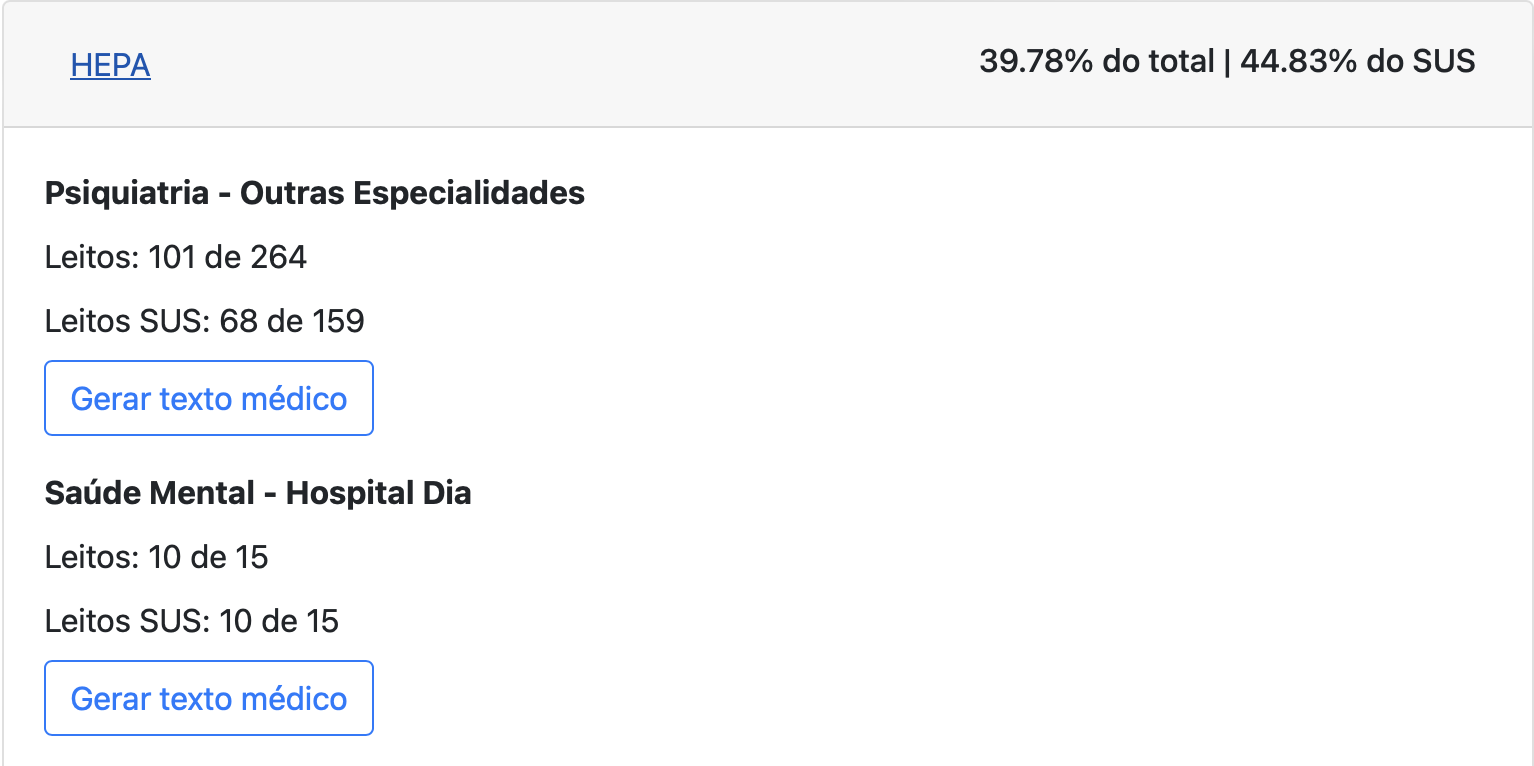
\includegraphics[width=\textwidth]{Capitulos/images/simul-result-1b.png}
    \caption{Estado dos leitos do hospital HEPA ao final do ultimo passo de simulação.}
    \label{fig:second}
\end{subfigure}
        
\caption{Resultados no primeiro e ultimo passo de simulação.}
\label{fig:simul-result-1}
\end{figure}

% \subsection{Geração de texto}
% Conforme apresentado na Seção~\ref{sec:geracao_texto}, para geração do texto médico é selecionado um paciente aleatório dentre os internados em uma especialidade de leito hospitalar especifica. O leito selecionado para geração do texto foi o de especialidade ``Saúde Mental'' do tipo de leito ``Hospital Dia''. A seguir é apresentado o texto gerado pela API da OpenAI e a descrição das características do paciente selecionado na Listagem~\ref{lst:select_paciente}. 

% \begin{spverbatim} 
% Lista de Problemas:

% Saúde Prévia: Não há histórico de doenças crônicas conhecidas.
% Medicações em Uso: Nenhuma medicação de uso contínuo registrada.
% Uso de Drogas: Nega tabagismo, consumo ocasional de álcool.
% HDA (História da Doença Atual):
% Paciente procurou atendimento devido a sintomas de ansiedade e depressão, com piora progressiva nos últimos meses.

% Subjetivo:
% Relatado pela paciente: Início gradual dos sintomas, incluindo tristeza persistente, insônia, falta de interesse em atividades diárias e pensamentos suicidas recentes.

% Objetivo:

% Estado Geral: Paciente apresenta-se abatida, com expressão facial entristecida.
% Avaliação do Sensório: Orientada no tempo, espaço e pessoa, porém com humor deprimido.
% Ausculta Cardíaca: Ritmo regular, sem sopros.
% Ausculta Pulmonar: Murmúrios vesiculares presentes bilateralmente.
% Abdômen: Sem alterações significativas à palpação.
% Extremidades: Sem edema, pulsos palpáveis bilateralmente.
% Resultados de Exames:

% Hemograma completo realizado em 05/04/2024: Dentro dos limites da normalidade.
% Eletrocardiograma (ECG) realizado em 05/04/2024: Sem anormalidades significativas.
% Impressão:
% Quadro sugestivo de transtorno depressivo maior com sintomas ansiosos, de gravidade moderada.

% Conduta:

% Encaminhamento para avaliação psiquiátrica completa.
% Prescrição de sertralina 50mg ao dia para tratamento da depressão, com acompanhamento ambulatorial.
% Encaminhamento para psicoterapia regular.
% Orientação para manutenção do acompanhamento médico e psicoterapêutico.
% Contato com familiar para apoio e monitoramento domiciliar.
% Registro realizado em 05/04/2024.
% \end{spverbatim}

% O texto gerado é coerente com a descrição da atividade solicitada ao modelo de geração de texto. No entanto, a informação sobre o tipo de leito associado ao paciente, seja privado ou SUS, não parece influenciar na geração do texto.

% \begin{listing}
% \begin{minted}[frame=single,
%                framesep=3mm,
%                linenos=true,
%                xleftmargin=21pt,
%                tabsize=4]{js}     
% {
%     'patient_id': 'b4ed248d-aaae-4d10-aad2-1f075a6a3003', 
%     'from_region': 'Teresópolis', 
%     'specialty': 'Saúde Mental', 
%     'type': 'Hospital Dia', 
%     'admission_time': 3, 
%     'return_frame': 3, 
%     'is_sus': True
% }
% \end{minted}
% \caption{Características do paciente na selecionado.} 
% \label{lst:select_paciente}
% \end{listing}

\section{Simulação 2}
A segunda simulação foi parametrizada com o mesmo hospital e especialidades de leitos hospitalares da simulação anterior, diferencia-se pela configuração da quantidade de internações durante o período de simulação. Com o objetivo de analisar um cenário de superlotação dos leitos hospitalares, foi considerado que o total de pacientes que chegam ao hospital durante o período de simulação fosse 10 vezes
%SO: 100 vezes seria 264*100 ou seja 26400...
a quantidade da capacidade dos leitos. Por exemplo, para o leito da especialidade ``Psiquiatria'' do tipo ``Outras Especialidades'' do hospital HEPA, estão disponíveis 264 espaços ao total, logo, na simulação serão encaminhados 2640 pacientes ao total para internação durante os 12 passos de simulação definido. A Figure~\ref{fig:simulacao2-a} ilustra a configuração do número de internações de pacientes na interface gráfica.

\begin{figure}
    \centering
    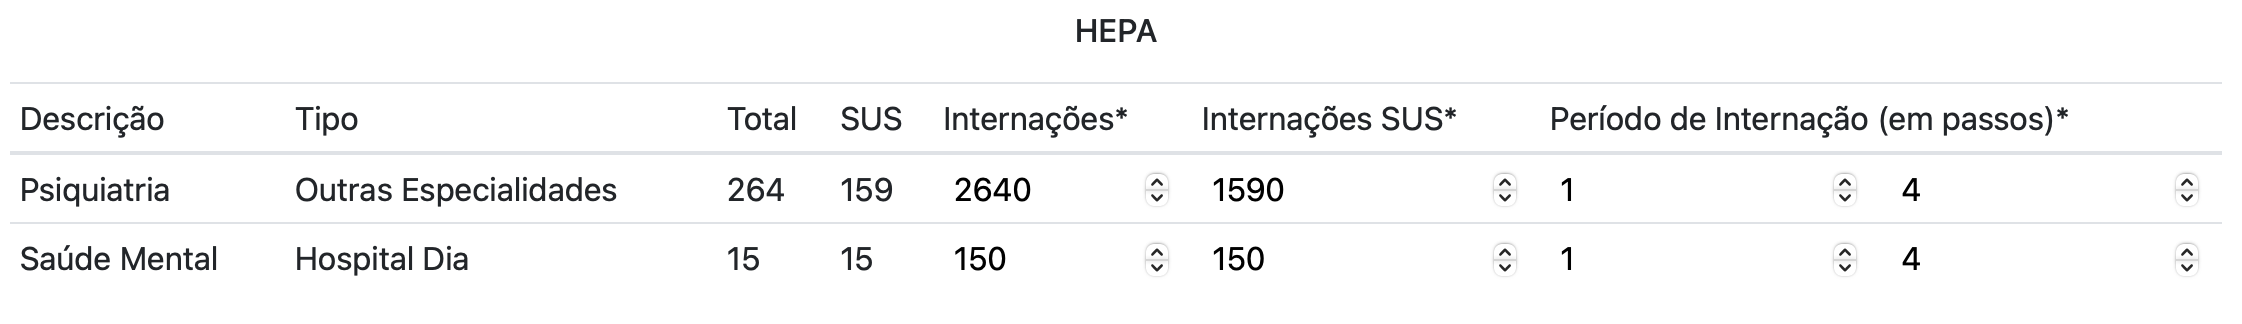
\includegraphics[width=\textwidth]{Capitulos/images/simulacao2-a.png}
    \caption{Configuração dos leitos do hospital HEPA na simulação.}%SO: falta caption na figura
    \label{fig:simulacao2-a}
\end{figure}

Realizada a simulação, pode-se observar que nos gráficos da Figura~\ref{fig:simulacao2} que dada a configuração utilizada, logo nos primeiros passos de simulação os leitos da especialidade ``Psiquiatria'' sofreram uma superlotação em ambos os tipos de leitos, privados e SUS. Já na Figura~\ref{fig:simulacao2b} os leitos da especialidade ``Saúde Mental'' superlotou no primeiro passo da simulação.

\begin{figure}
\centering
\begin{subfigure}{0.49\textwidth}
    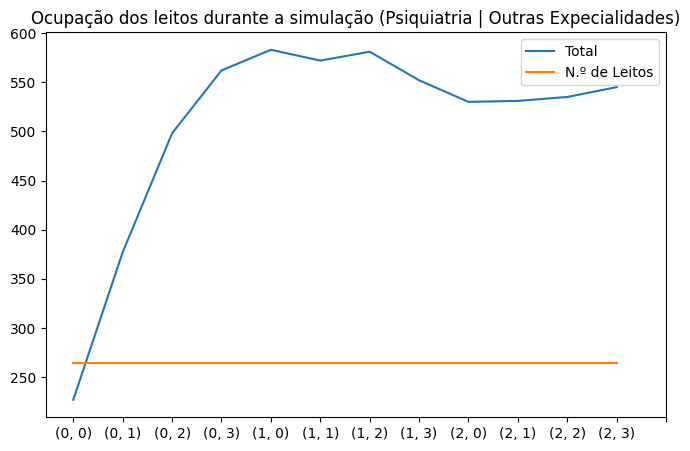
\includegraphics[width=\textwidth]{Capitulos/images/simulacao2-b.png}
    \caption{Ocupação dos leitos.}
    \label{fig:first}
\end{subfigure}
\hfill
\begin{subfigure}{0.49\textwidth}
    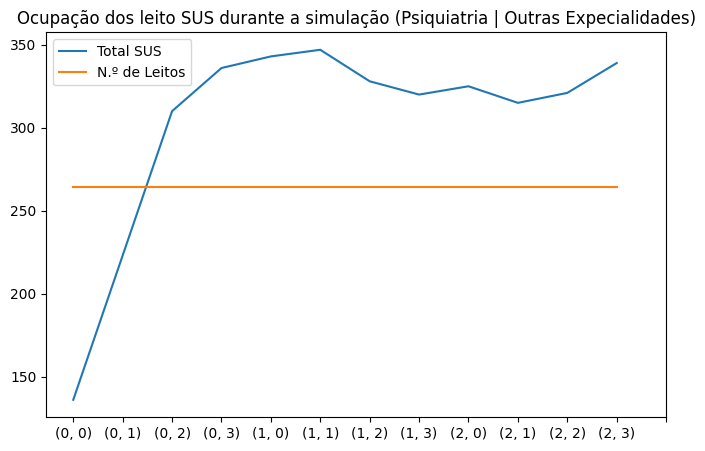
\includegraphics[width=\textwidth]{Capitulos/images/simulacao2-c.png}
    \caption{Ocupação dos leitos SUS.}
    \label{fig:second}
\end{subfigure}
        
\caption{Ocupação dos leitos durantes os passos de simulação para a especialidade ``Psquiatria'' do tipo ``Outras Especialidades'' do hospital HEPA.}
\label{fig:simulacao2}
\end{figure}

\begin{figure}
    \centering
    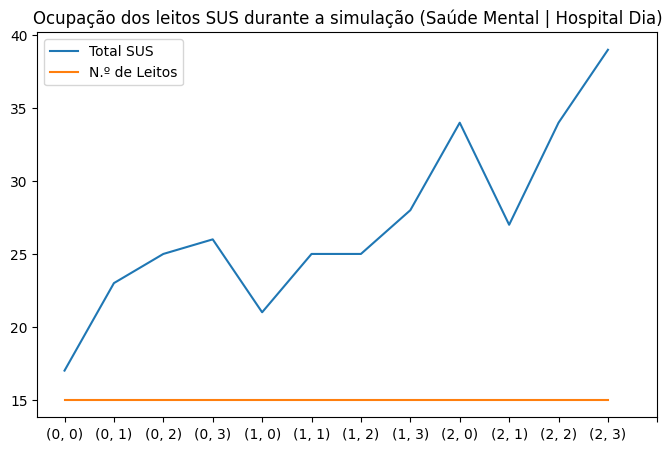
\includegraphics[width=0.5\textwidth]{Capitulos/images/simulacao2-d.png}
    \caption{Ocupação dos leitos SUS durantes os passos de simulação para a especialidade ``Saúde mental'' do tipo ``Hospital Dia'' do hospital HEPA.}
    \label{fig:simulacao2b}
\end{figure}

A Figura~\ref{fig:simulacao2-compare} apresenta uma comparação entre as diferentes simulações, apresentando o estado da ocupação dos leitos da região do hospital HEPA ao fim do primeira passo da simulação.

\begin{figure}
\centering
\begin{subfigure}{0.49\textwidth}
    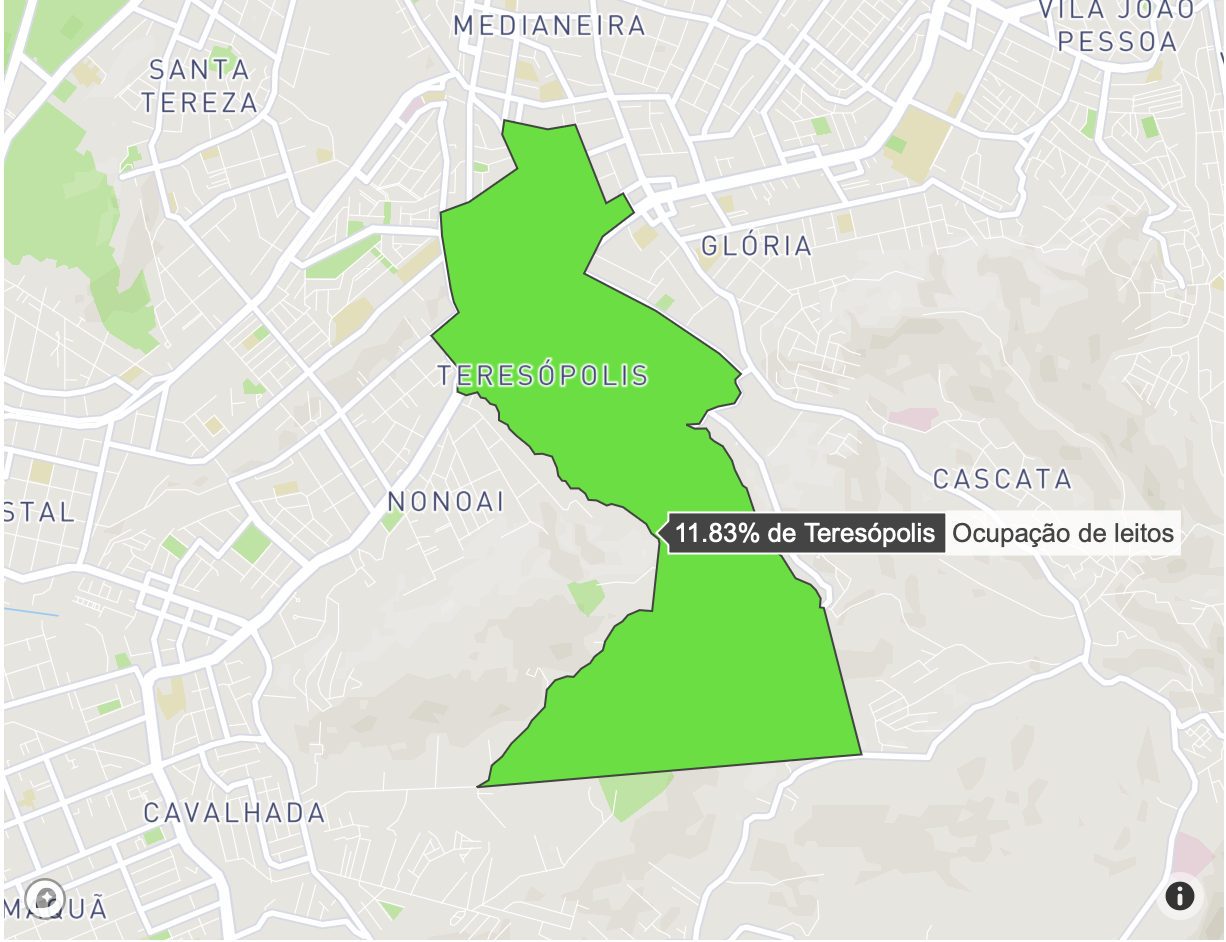
\includegraphics[width=\textwidth]{Capitulos/images/result2-compare-1.png}
    \caption{Ocupação dos leitos na simulação 1.}
    \label{fig:first}
\end{subfigure}
\hfill
\begin{subfigure}{0.49\textwidth}
    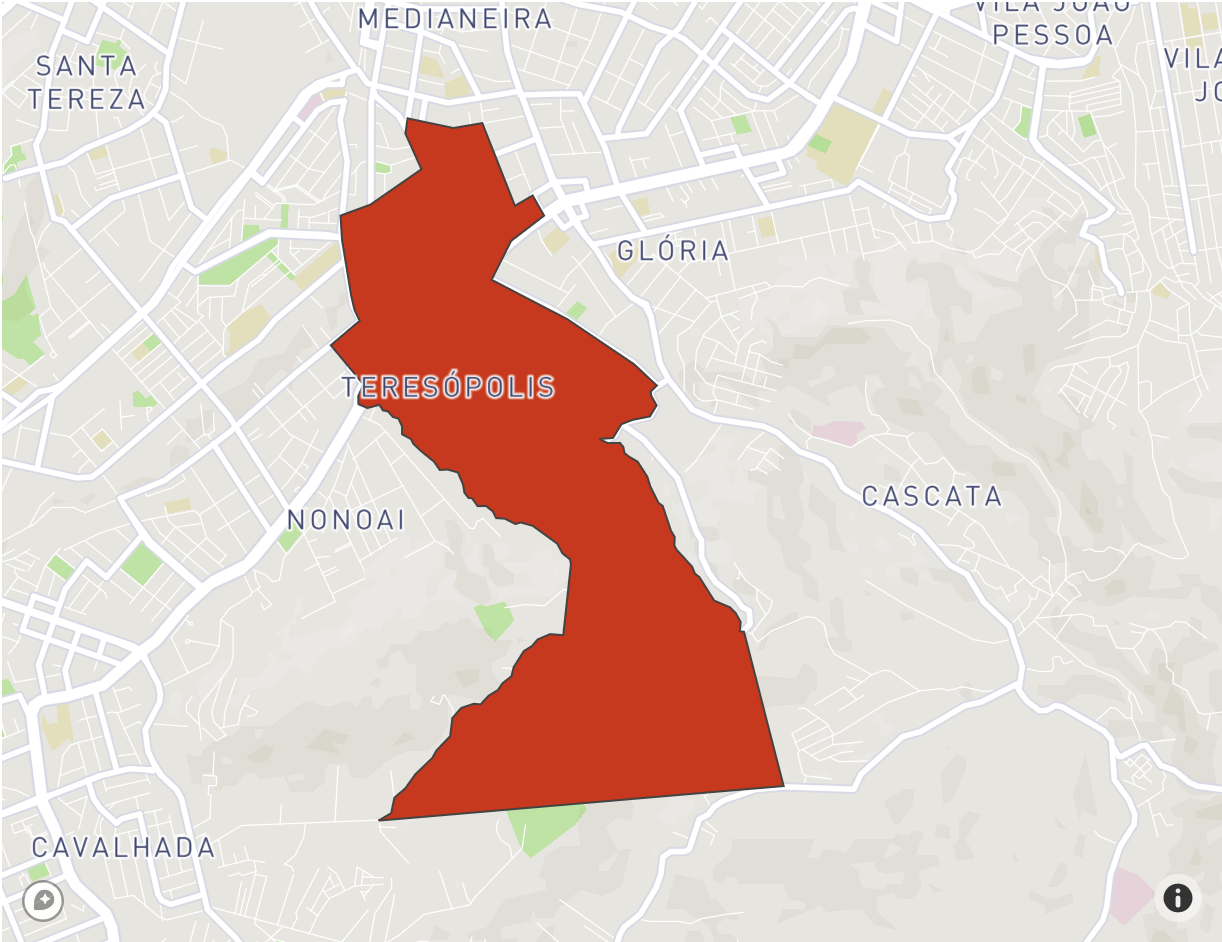
\includegraphics[width=\textwidth]{Capitulos/images/result2-compare-2.png}
    \caption{Ocupação dos leitos na simulação 2.}
    \label{fig:second}
\end{subfigure}
        
\caption{Comparação entre a ocupação dos leitos da região do hospital HEPA ao fim do primeiro passo de simulação nas simulações 1 e 2.}
\label{fig:simulacao2-compare}
\end{figure}

A simulação realizada indica que o modelo de simulação reproduz a superlotação dos conforme esperado, considerando a alta demanda de internações nos leitos hospitalares do HEPA configuradas pelo usuário na interface gráfica.

\section{Simulação 3}
A configuração utilizada na terceira simulação foi executada de forma a considerar dois hospitais no mesmo bairro, para isso, utilizamos os hospitais HEPA e Santa Ana, ambos localizados no bairro Teresópolis. Foi parametrizado que os hospitais teriam apenas uma especialidade de leito cada, a especialidade ``Psiquiatria'' do tipo ``Outras Especialidades''. Essa configuração foi criada com o objetivo de realizar uma comparação com o cenário da simulação anterior e entender o comportamento dos hospitais no caso de divisão dos pacientes entre eles. A Figura~\ref{fig:simulacao3a} ilustra a configuração dos dois hospitais na interface gráfica.

\begin{figure}
    \centering
    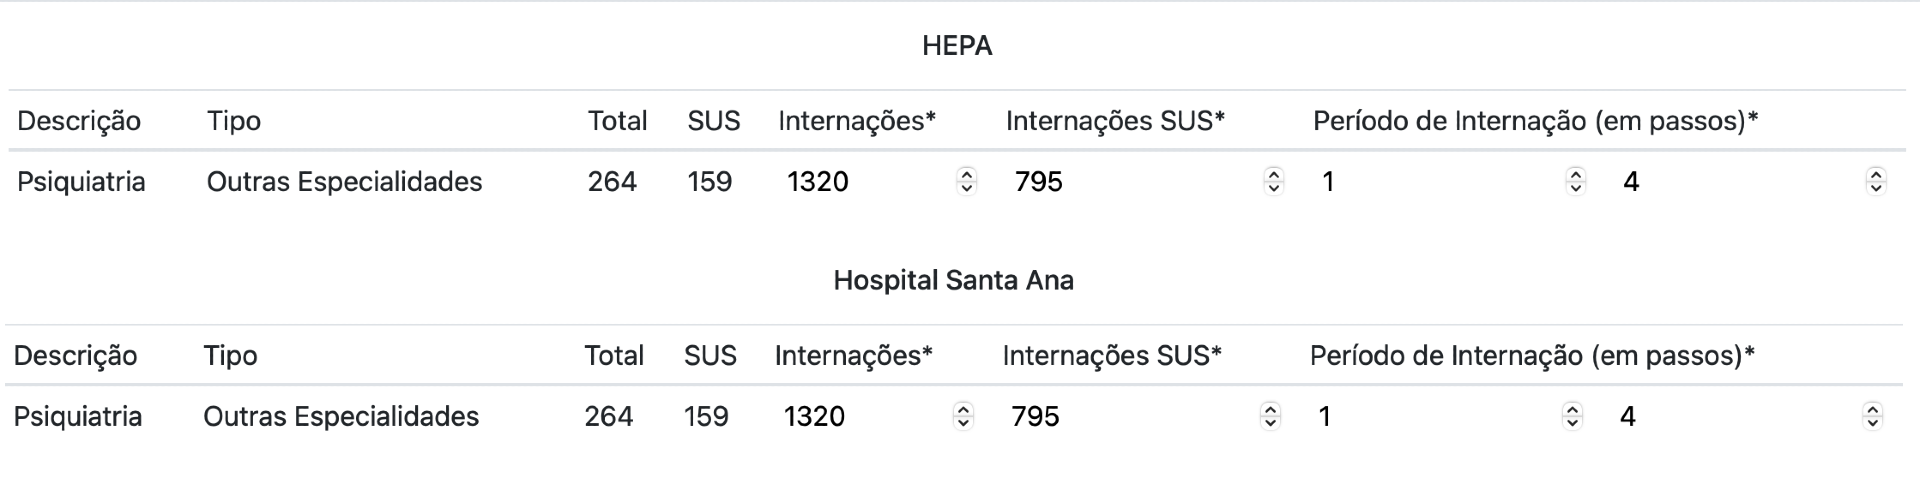
\includegraphics[width=\textwidth]{Capitulos/images/simulacao3-a.png}
    \caption{Configuração dos leitos dos hospitais HEPA e Santa Ana na simulação.}
    \label{fig:simulacao3a}
\end{figure}

A Figura~\ref{fig:simulacao3} apresenta os resultados dos passos de simulação para os dois hospitais considerando os leitos privados e SUS. Pode-se observar que a divisão dos pacientes entre os hospitais na simulação resulta em um tempo maior de execução até a superlotação do leito. Em comparação com a simulação anterior, o hospital HEPA (Figura~\ref{fig:simulacao3}(a)) que teve a superlotação dos leitos já no segundo passo de simulação, com a divisão entre os hospitais essa lotação dos leitos aconteceu apenas no passo 4 e voltou a ter leitos disponíveis no decimo primeiro passo, na simulação anterior os leitos permaneceram superlotados durante todos os passos de simulação seguintes. A Figura~\ref{fig:simulacao3}(b) ilustra o comportamento da ocupação dos leitos no hospital Santa Ana, onde observa-se um fluxo de ocupação semelhante ao do hospital HEPA e isso acontece devido aos dois hospitais possuírem as mesmas características em relação a essa especialidade de leito.

\begin{figure}
\centering
\begin{subfigure}{0.49\textwidth}
    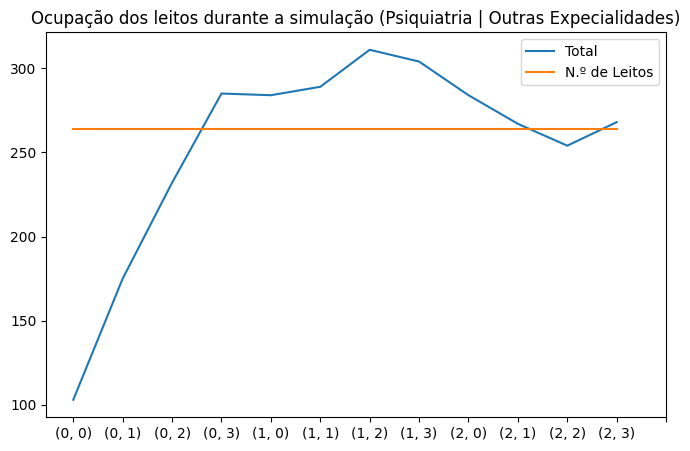
\includegraphics[width=\textwidth]{Capitulos/images/simulacao3-hepa.png}
    \caption{Ocupação dos leitos do hospital HEPA.}
    \label{fig:first}
\end{subfigure}
\hfill
\begin{subfigure}{0.49\textwidth}
    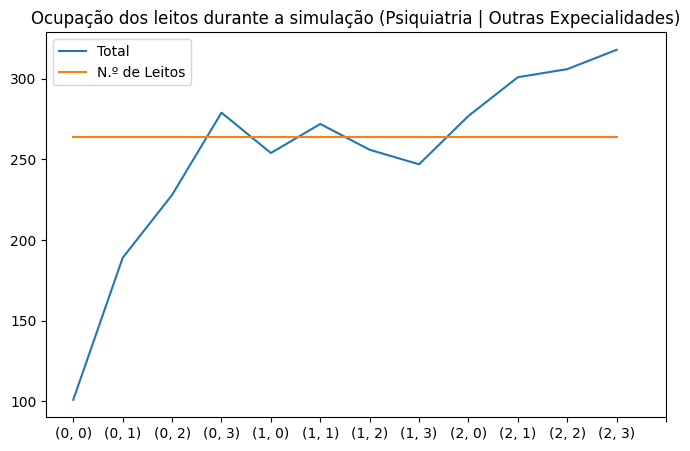
\includegraphics[width=\textwidth]{Capitulos/images/simulacao3-santaana.png}
    \caption{Ocupação dos leitos do hospital Santa Ana.}
    \label{fig:second}
\end{subfigure}
        
\caption{Ocupação dos leitos da especialidade “Psiquiatria” durante cada passo de simulação nos hospital HEPA e Santa Ana.}
\label{fig:simulacao3}
\end{figure}

Assim como no mundo real, inserir um novo hospital em uma região é uma possível abordagem para diminuir a ocupação dos leitos de um outro hospital próximo. Essa simulação demonstrou que o mesmo ocorre no ambiente de simulação ao disponibilizar um maior número de leitos para uma mesma demanda de internações apresentada na simulação anterior.

\section{Geração de Texto de Pacientes na Simulação}
Conforme apresentado na Seção~\ref{sec:geracao_texto}, para geração do texto médico é selecionado um paciente aleatório dentre os internados em uma especialidade de leito hospitalar especifica. Para a validação da geração de textos, foram selecionados pacientes internados nos leitos do hospital HEPA no sétimo passo da simulação da Seção~\ref{sec:simul1}. A Tabela~\ref{table:pacientes} mostra o percurso desses pacientes na simulação, sendo, a identificação do paciente (ID), a região de origem (Origem), a especialidade de leito em que foi internado (Leito), o passo de simulação em que chegou ao hospital (Chegada), em qual passo ele vai retornar para sua casa (Retorno) e se esta internado em um leito SUS ou privado (Setor).
 
\begin{table}[h!]
\centering
\begin{tabular}{ |l|l|l|l|l|l| } 
 \hline
 ID & Origem & Leito & Chegada & Retorno & Setor \\ 
 \hline
 f130ea18... & Teresópolis & Psiquiatria - Outras Especialidades & 4 & 8 & SUS \\ \hline
 3ee1981c... & Teresópolis & Psiquiatria - Outras Especialidades & 4 & 8 & SUS \\ \hline
 faab4cb8... & Teresópolis & Psiquiatria - Outras Especialidades & 4 & 8 & SUS \\ \hline
 b83792aa... & Azenha & Saúde Mental - Hospital Dia & 4 & 8 & SUS \\ \hline 
 f9d01e2f... & Santa Cecília & Saúde Mental - Hospital Dia & 4 & 9 & SUS  \\ \hline 
 85c85302... & Azenha & Saúde Mental - Hospital Dia & 3 & 8 & SUS \\ \hline
 \end{tabular}
\caption{Exemplos de pacientes internados no hospital HEPA no sétimo passo de simulação.}
\label{table:pacientes}
\end{table}

Para comparação da geração de texto médico em diferentes contextos utilizou-se de dois pacientes internados em especialidades de leitos distintos. Foram selecionados um paciente do leito de especialidade ``Psiquiatria'' do tipo ``Outras Especialidades'' e outro de ``Saúde Mental'' do tipo ``Hospital Dia''. A seguir é apresentado os textos médicos de evolução de pacientes gerados pelo modelo através da API da OpenAI. A geração do texto para o paciente internado em um leito de especialidade ``Psiquiatria'' do tipo ``Outras Especialidades'' retornou o seguinte resultado:

\begin{spverbatim}
SETOR DE EMERGÊNCIA PSIQUIÁTRICA

IDENTIFICADOR DO PACIENTE: f130ea18-5651-4eb7-b23b-ca8f2081d8ac

LISTA DE PROBLEMAS:
- Problemas de saúde prévios: Não há informações disponíveis sobre histórico 
médico prévio.
- Medicações em uso: Não há informações sobre uso prévio de medicamentos.
- Uso de drogas: Não há relato de uso de tabaco, álcool ou outras drogas.

HDA:
Paciente de 35 anos, sexo masculino, trazido pela família com queixa de 
agitação psicomotora, insônia e comportamento agressivo há 3 dias. Família 
relata que o paciente tem histórico de episódios similares, sem tratamento 
prévio.

SUBJETIVO:
Início súbito dos sintomas há 3 dias, segundo relato da família. 
Agressividade verbal e física, irritabilidade exacerbada, dificuldade para 
dormir, sem relato de alucinações ou delírios.

OBJETIVO:
- Estado geral: Paciente agitado, desorientado no tempo e no espaço.
- Sensório: Desorientado, reativo a estímulos verbais.
- Ausculta cardíaca: Ritmo cardíaco regular, sem sopros audíveis.
- Ausculta pulmonar: Murmúrio vesicular presente bilateralmente, sem ruídos 
adventícios.
- Abdômen: Sem alterações à palpação.
- Extremidades: Sem edema ou sinais de trauma.

EXAMES:
- Hemograma completo (05/04/2024): dentro dos valores de referência.
- Bioquímica sanguínea (05/04/2024): dentro dos valores de referência.

IMPRESSÃO:
Quadro compatível com episódio agudo de transtorno psicótico agudo, 
necessitando de avaliação psiquiátrica urgente.

CONDUTA:
1. Encaminhamento para avaliação psiquiátrica emergencial.
2. Sedação com benzodiazepínico conforme protocolo.
3. Manter em observação na emergência até avaliação psiquiátrica.
4. Orientações à família sobre a necessidade de acompanhamento psiquiátrico 
regular.
5. Solicitação de internação psiquiátrica compulsória, se necessário, de 
acordo com legislação vigente.
\end{spverbatim}

Após, o mesmo procedimento é aplicado para o paciente internado no leito de especialidade ``Saúde Mental'' do tipo ``Hospital Dia'' e o resultado do texto gerado foi o seguinte:

\begin{spverbatim}
SETOR DE SAÚDE MENTAL - HOSPITAL DIA

IDENTIFICADOR DO PACIENTE: f9d01e2f-de4e-430e-a663-b0454fda937d

LISTA DE PROBLEMAS:
- Problemas de saúde prévios: Transtorno de ansiedade generalizada.
- Medicações em uso: Sertralina 50mg/dia.
- Uso de drogas: Não há relato de tabagismo, consumo de álcool ou outras 
drogas.

HDA:
Paciente de 42 anos, sexo feminino, busca atendimento devido a piora dos 
sintomas de ansiedade e insônia nas últimas semanas, com dificuldade para 
realizar as atividades diárias.

SUBJETIVO:
Sintomas de ansiedade exacerbados nas últimas semanas, relatando preocupações 
excessivas, inquietação, dificuldade de concentração e irritabilidade. Refere 
insônia persistente, com dificuldade para iniciar e manter o sono.

OBJETIVO:
- Estado geral: Paciente aparenta ansiedade, porém coopera com o exame.
- Sensório: Alerta e orientada quanto ao tempo, espaço e pessoa.
- Ausculta cardíaca: Ritmo cardíaco regular, sem sopros audíveis.
- Ausculta pulmonar: Murmúrio vesicular presente bilateralmente, sem ruídos 
adventícios.
- Abdômen: Sem alterações à palpação.
- Extremidades: Sem edema ou sinais de trauma.

EXAMES:
- Hemograma completo (05/04/2024): dentro dos valores de referência.
- Bioquímica sanguínea (05/04/2024): dentro dos valores de referência.

IMPRESSÃO:
Transtorno de ansiedade generalizada, com piora dos sintomas interferindo 
nas atividades diárias.

CONDUTA:
1. Ajuste na dose de sertralina para 75mg/dia.
2. Encaminhamento para acompanhamento psicológico regular.
3. Orientações sobre técnicas de relaxamento e manejo do estresse.
4. Reavaliação em duas semanas para monitoramento da resposta ao tratamento.
\end{spverbatim}

Os textos gerados se demonstram coerentes com a descrição da atividade solicitada ao modelo de geração de texto. No entanto, a informação sobre o setor do leito associado ao paciente, seja privado ou SUS, não parece influenciar na geração do texto, já a especialidade, tipo de leito e o identificador do paciente são relevantes para o resultado do texto gerado. Os textos gerados estão associados a descrição de um único paciente para cada texto, assim, enfatizando a possibilidade de individualização da população do LODUS a partir do \textit{plugin} desenvolvido.